
\section{Foundations of Data Flow Analysis}


$\leq$ means more conservative, but not means subset.


\subsection{Transfer Functions}





\subsubsection{monotonicity}

% \begin{tcolorbox}
% efjer
% \end{tcolorbox}

\begin{note}{Monotone framework doesn't mean $ f(x) \leq x$}
For example, reaching definition for just one definition \texttt{a=1} in a BasicBlock(\texttt{BB1}).  \[IN(BB1) = \{\} = x = \top , OUT(BB1) = {a} = f(x) \]
However, $x = \top \leq  f(x)$
\end{note}

\subsubsection{Distributivity}

Not a requirement.

\begin{definition}{Distributivity}

A framework $F,V, \wedge$ is \emph{distributive} is and only if 

\[f(x \wedge y)=f(x) \wedge f(y)\]

which means applying $f$ to the merge input is equal to applying $f$ individually then merge result. 
\end{definition}

Reaching definition is distributive.


Constant Propagation is not distributive. 
\begin{figure}[h]
    \centering
    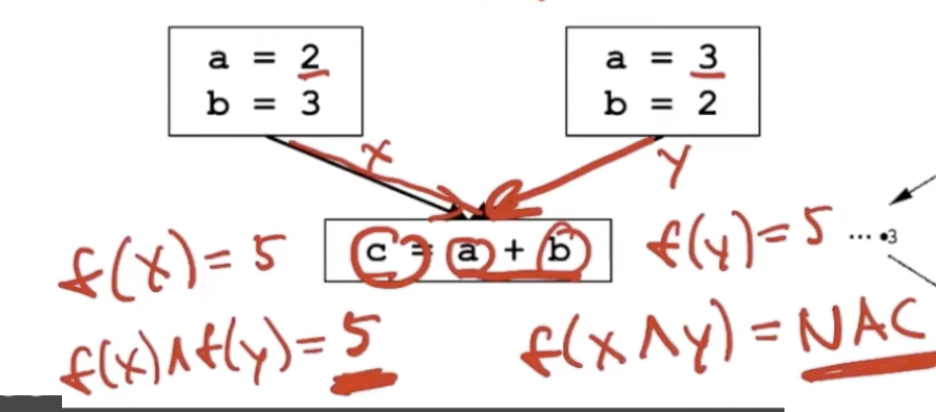
\includegraphics[width=0.2\textwidth]{CDp.png}
    \caption{}
    \label{fig:p15}
\end{figure}

\subsection{Data Flow Analysis}

\begin{definition}{Definition}
Let $f_1, \dots , f_m \in F$, where $f_i$ is the transfer function for node $i$. $f_p=f_{n_k} \cdot \ldots \cdot f_{n_1}$, where $p$ is a path through nodes $n_1  \cdot \ldots \cdot n_k$. $f_p =$ identify function, if $p$ is an empty path.
\end{definition}

\subsubsection{Precision}

Ideally for each node n, the IN should be $ \wedge f_{p_i}(\top)$ for all possibly executed path $p_i$ reaching n. But determining all possible executed paths is undecidable. Look at the example shown in \ref{fig:p20}.


\begin{figure}[h]
    \centering
    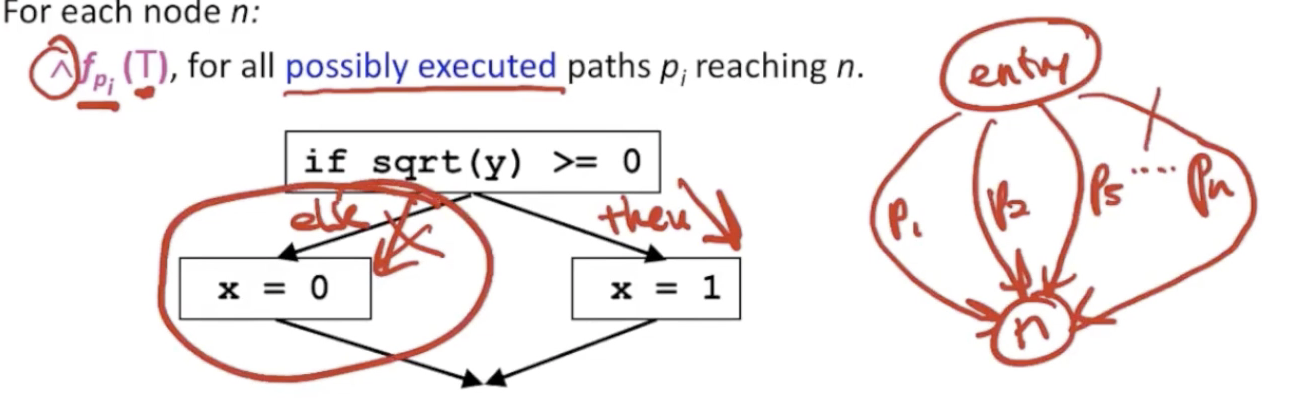
\includegraphics[width=0.2\textwidth]{p20.png}
    \caption{}
    \label{fig:p20}
\end{figure}

So in reality,  we will conservatively include some paths that will never be executed. From a correctness standpoint, this is fine because we will just get an more conservative answer.

\subsubsection{Meet-Over-Path(MOP)}

\begin{definition}{MOP}
For each node n, MOP(n) = $ \wedge f_{p_i}(\top)$ for all possibly executed path $p_i$ reaching n. 

Strictly speaking, MOP considers more paths than necessary, which means 

\[ \textit{MOP = Perfect-Solution} \wedge  \textit{Solution-to-Unexecuted-Paths.}\]

So 

\[ MOP \leq \textit{ Perfect-Solution} \]

MOP is more conservative. 

\end{definition}



\subsection{Solving Data Flow Equations}

Any solution that satisfies equations is a Fixed Point Solution(FP).


\subsubsection{Iterative algorithm }

If framework is monotone and algorithm coverges, then it computes Maximum Fixed Point(MFP).


FP $\leq$ MFP $\leq$ MOP $\leq$ Perfect-solution


Reaching Definition example:
\begin{figure}[h]
    \centering
    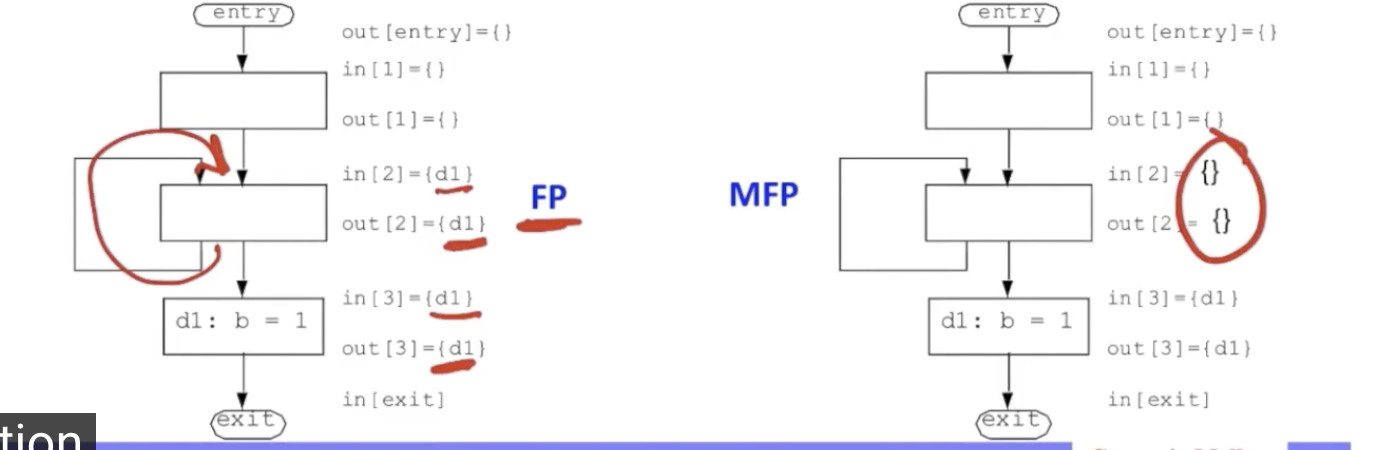
\includegraphics[width=0.2\textwidth]{p21.png}
    \caption{}
    \label{fig:p21}
\end{figure}




\subsection{Precision}

If data flow framework is distributive, then if the algorithm converges, $IN[b] = MOP[b]$

A Monotone but not distributive example: Constant Propagation.(Behaves as if there are additional paths)



\subsection{Convergence}
Properties are needed to guarantee convergence:

\begin{itemize}
    \item monotone
    \item finite descending chain
\end{itemize}



\subsection{Speed of Convergence}

\subsubsection{Reverse Post order}

\begin{figure}[h]
    \centering
    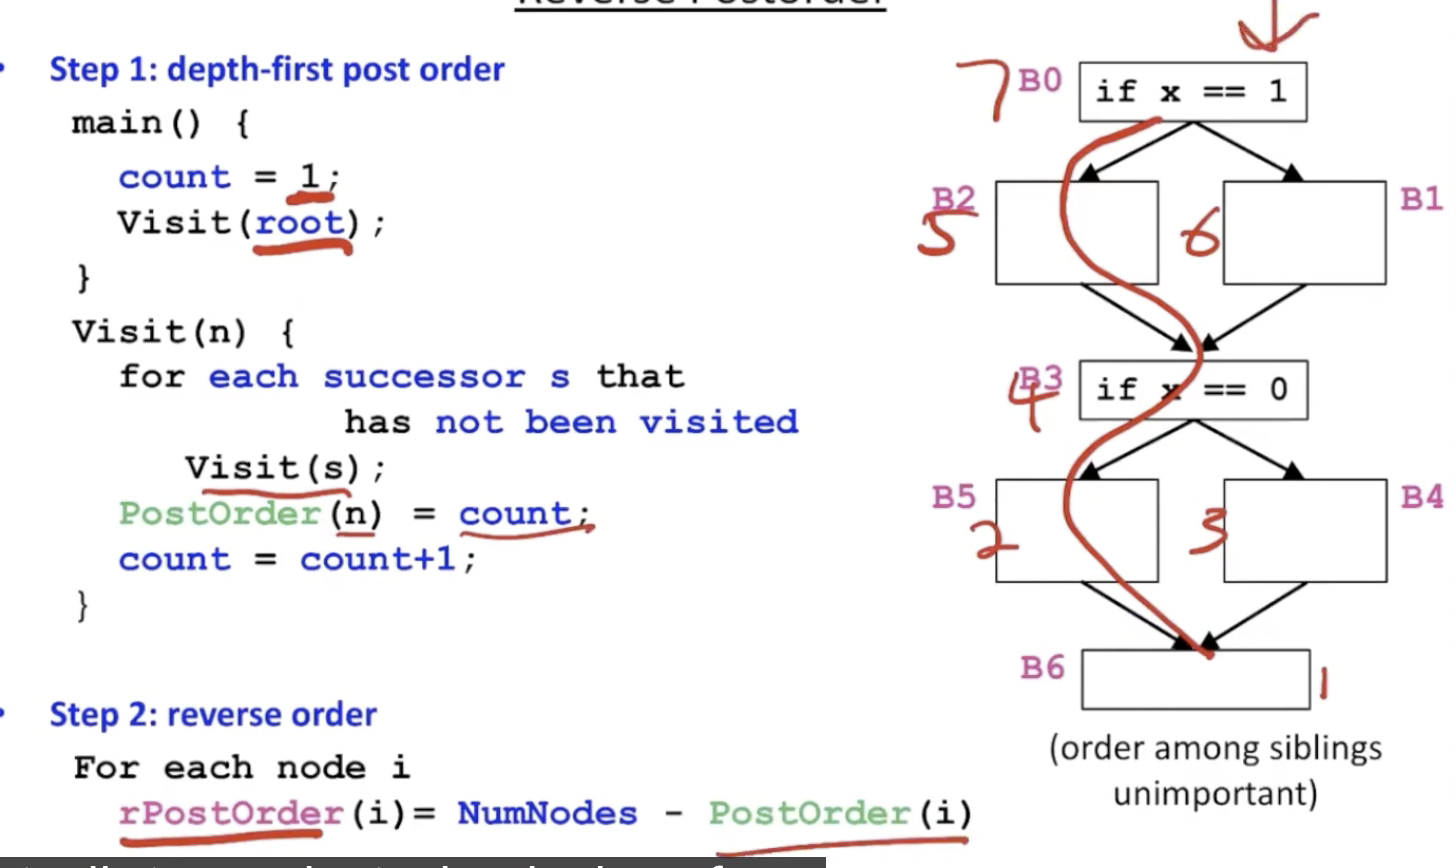
\includegraphics[width=0.2\textwidth]{p22.png}
    \caption{}
    \label{fig:p22}
\end{figure}


\subsubsection{Depth-First Iterative Algorithm(forward)
}



\begin{figure}[h]
    \centering
    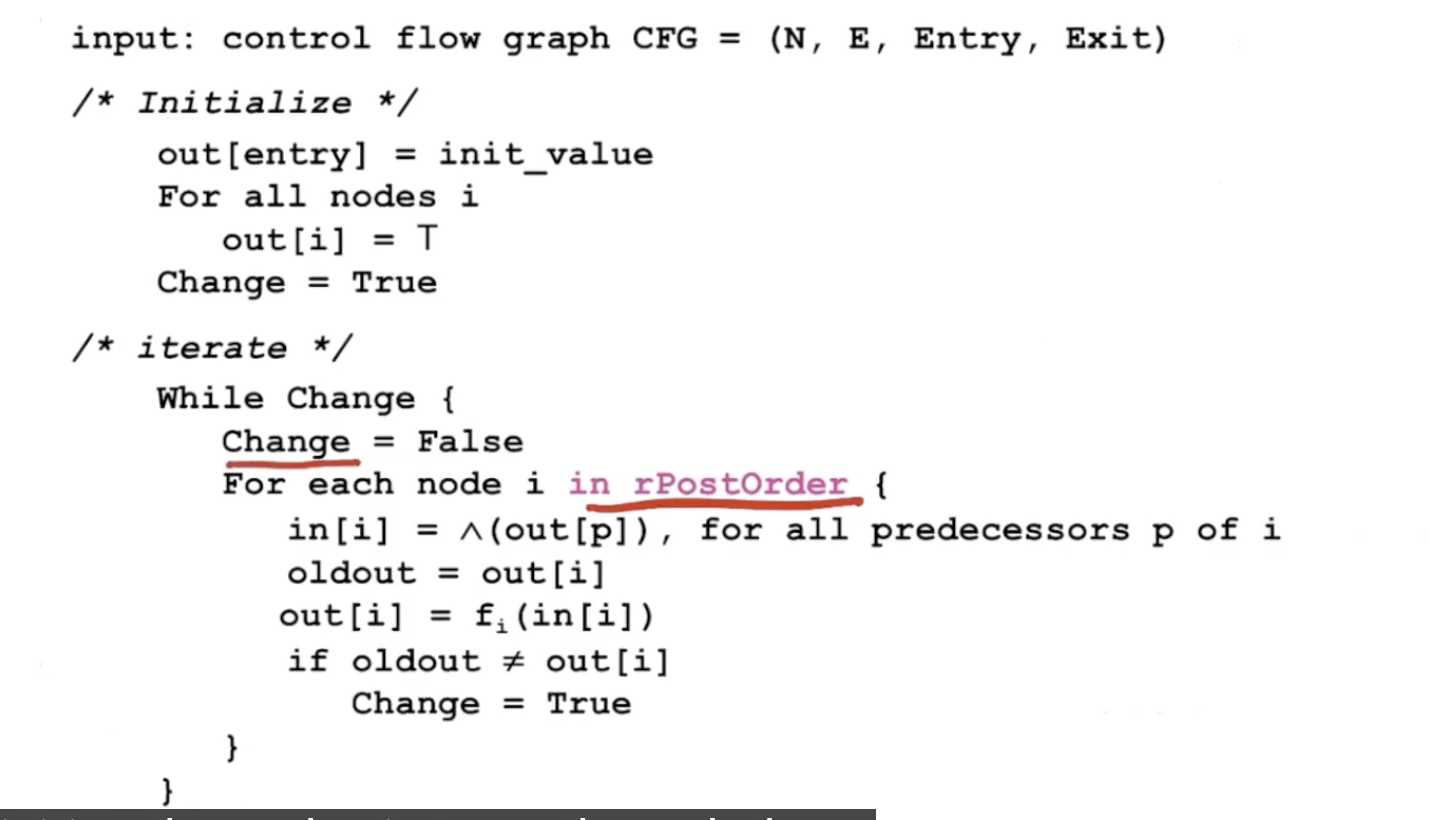
\includegraphics[width=0.2\textwidth]{p23.png}
    \caption{}
    \label{fig:p23}
\end{figure}


\subsubsection{Cost}

Number of iterations = number of back edges in any acyclic path +2 




